\documentclass[a4paper,pt11,oneside]{book}
\usepackage[latin1]{inputenc}
\usepackage[italian]{babel}
\usepackage[T1]{fontenc}
\usepackage[utf8x]{inputenc}
\usepackage{listings}
\usepackage{color}

\definecolor{dkgreen}{rgb}{0,0.6,0}
\definecolor{gray}{rgb}{0.5,0.5,0.5}
\definecolor{mauve}{rgb}{0.58,0,0.82}
\definecolor{light-gray}{gray}{0.25}

\lstset{
  language=Java,
  aboveskip=3mm,
  belowskip=3mm,
  showstringspaces=false,
  columns=flexible,
  basicstyle={\footnotesize\ttfamily},
  numberstyle={\tiny},
  numbers=left,
  keywordstyle=\color{blue},
  commentstyle=\color{dkgreen},
  stringstyle=\color{mauve},
  breaklines=true,
  breakatwhitespace=true,
  tabsize=3
}
\linespread{1.5}
\usepackage{graphicx}
\graphicspath{ {images/} }
\title{
\huge
\textbf{Spazi ~Aule con Framework ~GWT}\\
{
\includegraphics[scale=2]{university.jpg}}}
\author{Ferrari~Nico}
\begin{document}
\maketitle
\renewcommand{\contentsname}{Indice}
\tableofcontents
\listoffigures

\chapter{Introduzione}
Nello sviluppo tecnico delle applicazioni web e mobile la scelta del framework e della modalità di sviluppo del progetto, che si adatta meglio alle esigenze di mercato del cliente, è un elemento critico che deve essere valutato con grande attenzione visti gli impatti sul business nel medio e breve termine.

Quando si parla di framework si intende un'architettura logica di supporto (spesso un'implementazione logica di un particolare design pattern) su cui un software può essere progettato e realizzato, spesso facilitandone lo sviluppo da parte del programmatore.

Oggi sul mercato esistono diversi tipi di framework, ognuno con caratteristiche e vantaggi differenti. Ciascuno di essi supporta uno o più sistemi operativi, ma non è detto che un framework possa supportare completamente le funzionalità richieste da un’applicazione e da un progetto.

Il lavoro di tesi svolto si pone come obiettivo lo sviluppo in team di un'applicazione web che mette a disposizione degli utenti una visione chiara e completa dell'occupazione delle aule negli spazi universitari. L'applicazione si propone quindi di rendere un servizio sia basato sulla semplice e veloce consultazione delle informazioni riguardanti lo stato delle aule universitarie, sia la manipolazione di tali informazioni.

Oltre all'applicazione web, è stata creata un'applicazione Android per avere un sistema di monitoraggio degli spazi anche su dispositivi mobili.

Per lo sviluppo di questo progetto sono stati utilizzati diversi framework per coprire tutte le richieste e necessità.\\ Nella tesi tratterò esclusivamente la web app, la parte di progetto su cui mi sono soffermato principalmente in fase di sviluppo.
\newpage La tesi è composta da 4 capitoli:
\begin{itemize}
\item Il primo capitolo descrive gli strumenti e tecnologie utilizzate durante la fase di progettazione e sviluppo dell'applicazione;
\item il secondo capitolo espone il progetto stesso e mostra le sue funzionalità nel dettaglio;
\item nel terzo capitolo varrano mostrate le problematiche incontrate e i benefici portati dalle tecnologie usate;
\item infine verranno riportati in appendice i requisiti in forma tabellare e alcune informazioni utili per la manutenzione del sistema.
\end{itemize}

\chapter{Strumenti utilizzati}
\section{JAVA}
Il  linguaggio Java  \`e  un  linguaggio  di  programmazione  orientato  agli  oggetti,  creato  da  James 
Gosling  e  altri  ingegneri  di  Sun  Microsystems.  Il  gruppo  inizi\`o  a  lavorare  nel  1991,  il  linguaggio 
inizialmente si chiamava Oak. Il nome fu successivamente cambiato in Java a causa di un problema di  copyright  (il  linguaggio  di  programmazione  Oak  esisteva  gi\`a nel  1991).  Java  fu  annunciato ufficialmente il 23 maggio 1995 a SunWorld. La piattaforma di programmazione Java \`e fondata sul 
linguaggio  stesso,  sulla  Java  Virtual Machine  (JVM)e  sulle  API.  Java  \`e  un  marchio  registrato  di Sun Microsystems.

\subsection{Panoramica del linguaggio JAVA}
Java venne creato per soddisfare quattro scopi: 
\begin{itemize}
\item essere orientato agli oggetti
\item essere indipendente dalla piattaforma
\item contenere strumenti e librerie per il networking
\item essere progettato per eseguire codice da sorgenti remote in modo sicuro
\end{itemize}
\subsection*{Orientamento agli oggetti}
Java \`e un linguaggio object-oriented. La programmazione orientata agli oggetti (OOP, Object Oriented Programming) \`e un paradigma di programmazione che permette di definire oggetti software in grado di interagire gli uni con gli altri attraverso lo scambio di messaggi.  Questi oggetti, come nella vita pratica hanno propriet\`a rappresentate da valori, e qualit\`a o meglio metodi: 
ci\`o che sanno fare questi oggetti.

La programmazione ad oggetti \`e particolarmente adatta nei contesti in cui si possono definire delle relazioni di interdipendenza tra i concetti da modellare (contenimento, uso, specializzazione). 

Tra i vantaggi della programmazione orientata agli oggetti abbiamo:
\begin{itemize}
\item fornisce un supporto naturale alla modellazione software degli oggetti del mondo reale o del modello astratto da riprodurre
\item permette una pi\`u facile gestione e manutenzione di progetti di grandi dimensioni
\item permette una pi\`u facile gestione e manutenzione di progetti di grandi dimensioni
\item l'organizzazione del codice sotto forma di classi favorisce la modularit\`a e il riuso di codice
\end{itemize}
\subsection*{Indipendenza dalla piattaforma}
L'indipendenza dalla piattaforma significa che l’esecuzione di programmi scritti  in  Java  deve  avere  un  comportamento  simile 
in contesti di esecuzione diversi. Per raggiungere questo obiettivo il codice Java viene compilato in un linguaggio intermedio bytecode. Il bytecode \`e un insieme di istruzioni altamente ottimizzate eseguibili dalla Java Virtual Machine(JVM), disegnata inizialmente come interprete per tale linguaggio.

La traduzione di un programma Java in bytecode rende molto piu semplice l'esecuzione di un programma in una vasta gamma di ambienti perch\`e solo la JVM deve essere implementata per ogni piattaforma.
\subsection*{Esecuzione sicura del codice remoto}
La piattaforma Java ha caratteristiche progettate per aumentare la sicurezza delle applicazioni Java:
\begin{itemize}
\item \textbf{La JVM:}\\
La JVM esegue una verifica del bytecode prima di eseguirlo per prevenire l'esecuzione di operazioni non sicure e per far rispettare vincoli a runtime. La piattaforma non permette ai programmi di eseguire alcune operazioni insicure e controlli manuali sull'allocazione e deallocazione della memoria.
\item \textbf{Il Security Manager:}\\
La piattaforma fornisce un security manager che permette agli utenti di eseguire codice bytecode inaffidabile in un ambiente "sandbox" progettato per proteggerli da software pericoloso o scritto male evitando che il tale codice abbia accesso ad alcune caratteristiche e API della piattaforma.
Il security manager permette di assegnare ai programmi Java una firma digitale in modo tale che l'utente possa scegliere di dare i privilegi a software con firma digitale valida proveniente da entità di fiducia.
\item \textbf{Le API:}\\
Viene fornita una serie di API orientate alla sicurezza, come algoritmi standard di crittografia,autenticazione e protocolli di comunicazione sicuri.
\end{itemize}

\subsection{La piattaforma JAVA}
La  piattaforma  Java  \`e  una  piattaforma  solo software eseguita sopra ad  una  piattaforma hardware di base che pu\`o essere un computer, una tv, un telefono cellulare, una smart card, ecc...
\\ La piattaforma Java \`e composta da due blocchi: 
\begin{itemize}
\item la Java Virtual Machine (JVM)
\item la Java Application Program Interface (API)
\end{itemize} 
La JVM \`e  la  base  della  piattaforma  Java, mentre la Java API \`e  una  collezione  di componenti software pronti all’uso per losvolgimento dei pi\`u disparati compiti.
\subsection*{Java Virtual Machine} 
La JVM consiste in:
\begin{description}
\item [Class loader:]
carica le classi che formano il bytecode, sia dell'applicazione Java, sia delle API Java necessarie per l'esecuzione da parte dell'interprete Java.

\item [Class verifier:]
controlla che il bytecode sia valido, che non superi i limiti superiori o inferiori dello stack, assicura non esegua aritmetica dei puntatori (che potrebbe potenzialmente portare ad una violazione di memoria). Se il bytecode passa tutti questi controlli, pu\`o essere eseguito dall'interprete.

\item [Interprete Java:] 
pu\`o essere di varie forme: pu\`o essere un modulo software che interpreta il bytecode in una sola volta oppure pu\`o fare uso di un compilatore just-in-time (JIT, o Just-In-Time compiler) che traduce a run-time il bytecode in codice nativo della macchina ospitante e lo salva in memoria durante l'esecuzione. \`E anche possibile utilizzare un sistema "misto", in cui il JIT viene applicato solo alle porzioni di codice del programma utilizzate pi\`u frequentemente, mentre il resto viene interpretato.
\end{description}

\subsection*{API Java}
Le API Java raccolgono una gran quantit\`a di componenti disponibili per scrivere applicazioni di qualsiasi genere. Per questo motivo la piattaforma Java \`e disponibile in tre configurazioni a seconda dell'uso che se ne vuole fare:
\begin{itemize}
\item \textbf{Standard Edition.} Fornisce API per le esigenze pi\`u comuni, che permette di scrivere applicazioni stand-alone, applicazioni client e server in un contesto di reti di computer, applicazioni per accesso a database, applicazioni per il calcolo scientifico e di altro tipo.
\item \textbf{Enterprise Edition.} Permette di scrivere applicazioni distribuite.
\item \textbf{Micro Edition.} Permette di scrivere applicazioni per i terminali mobili e, pi\`u in generale, per i dispositivi dotati di poche risorse computazionali (telefoni cellulari, palmari, smart cards ed altri).
\end{itemize}

\section{Framework Hibernate}
La gestione della persistenza \`e un argomento delicato nella progettazione di applicazioni software.
Lo sviluppo di applicazioni Object-Oriented che utilizzano un DBMS relazionale per immagazinare i dati in memoria secondaria \`e uno scenario molto comune. Ci\`o che rende complessa la costruzione dello strato di persistenza \`e il problema dell'object/relational impedence mismatch, ovvero la discrepanza tra il paradigma Object-Oriented e il paradigma relazionale.\\
Fondamentalmente, gli oggetti fanno riferimento ad altri oggetti e perci\`o danno forma ad un grafo, a differenza degli gli schemi relazionali, che hanno invece una struttura tabellare e basati sull'algebra relazionale che definisce insiemi di tuple. La conversione di tuple in strutture a grafo spesso richiede molto tempo e pu\`o risultare difficile, infatti, viene anche descritta "Vietnam of Computer Science".
Questo problema pu\`o esser diviso in pi\`u parti:
\begin{itemize}
\item \textbf{Struttura, Ereditariet\`a, Interfaccia e Polimorfismo}:\\
Una classe specifica gli attributi e i metodi che devono avere gli oggetti che appartengono ad essa e pu\`o anche far parte di una gerarchia (concetto di ereditariet\`a).
Il modello relazionale non contempla il concetto di “classe” di oggetti e non fornisce una analogia per le gerarchie, interfacce e polimorfismo.  
\item \textbf{Granularit\`a dei tipi di dato}:\\
Tipi di dati composti sono tipicamente  rappresentati nei linguaggi OO mediante classi di oggetti, mentre nel modello relazionale non si prevede alcun meccanismo per la definizione di tipi di dato composti. 
\item \textbf{Incapsulamento}:\\
Lo stato di un oggetto \`e incapsulato ed \`e accessibile attraverso i metodi. Lo stato di una riga di una tabella non contempla questo aspetto e pu\`o essere modificato in maniera diretta.
\item \textbf{Identit\`a}:\\
Gli oggetti esistono indipendentemente dal loro stato. Essi possono essere identici o uguali. Se due oggetti sono identici, essi sono lo stesso oggetto. Se sono uguali, essi contengono gli stessi valori. Nel modello relazionale, invece, le righe sono identificate solo dai valori che esse contengono.
\item \textbf{Associazioni}:\\
Il modello relazionale contempla solo un tipo di associazione: l'utilizzo di una chiave esterna, che si riferisce ad una chiave primaria di un'altra tabella. Il paradigma Object-Oriented contempla diverse tipologie di associazione: uno a uno, uno a molti, molti a molti.
\item \textbf{Coesione}:\\
Tutte le propriet\`a di un oggetto sono contenuto all'interno di esso. Invece, le relazioni che corrispondono ad una stessa entit\`a possono essere stati suddivisi in pi\`u tabelle (fase di ristrutturazione dello schema logico)
\end{itemize}
Il problema dell'impedence mismatch deve essere analizzato e risolto nel modo opportuno in fase di progettazione. 

Un altro aspetto molto importante nella gestione della persistenza \`e l'interazione tra lo strato di business logic e lo strato di persistenza.
In applicazioni Java la comunicazione con la base di dati avviene utilizzando API specifiche come ODB (Open Database Connectivity) o JDBC(Java Database Connectivity). 
Una delle strategie pi\`u valide e utilizzate \`e l'uso del pattern Data Access Object (DAO) per la creazione di oggetti che costituiscono uno strato di comunicazione con la base di dati. 
La realizzazione dei DAO avviene usando API JDBC
per rendere disponibili le operazioni CRUD(Create Read Update Delete) allo strato di logica applicativa. I DAO incapsulano l'accesso alla base di dati e permettono di gestire la maggior parte degli scenari ma la loro realizzazione necessita di una conoscenza dettagliata della base di dati.
Altri strategie fanno uso della serializzazione, di object oriented database systems oppure dell'Object-Relational Mapping che consiste nel mappare le classi di dominio dell'applicazione su una base di dati relazionale. 

\subsection{Object/Relational Mapping}
L'Object/Relational Mapping (ORM) \`e una tecnica di programmazione che favorisce l'integrazione di sistemi software aderenti al paradigma della programmazione orientata agli oggetti con sistemi RDBMS.
Attraverso questo mezzo ogni oggetto viene reso persistente nel database tramite l'inserimento di nuovi record i cui campi contengono i valori degli attributi dell'oggetto stesso. Si viene quindi a creare la relazione tra oggetto Java e tabella SQL. Una soluzione ORM consiste di quattro componenti caratteristici:

\begin{enumerate}
\item Una API per eseguire le operazioni CRUD sugli oggetti delle classi del modello.
\item  Un linguaggio  o una API  per specificare query che fanno riferimento alle classi e alle propriet\`a delle classi.
\item Uno srumento per la specifica del mapping mediante metadata.
\item Una tecnica per l'implementazione di ORM  per interagire con oggeti transazionali al fine di eseguire funzioni di ottimizzazione.
\end{enumerate}

L'associazione fisica tra la classe e la tabella viene ottenuta mediante l'utilizzo di file di descrizione (detti file di mapping), in cui si specificano le modalit\`a di conversione tra gli attributi dell'oggetto e i campi della tabella. In definitiva i principali vantaggi derivanti dall'uso di una soluzione ORM sono:

\begin{itemize}
\item Snellimento della parte di codice riservata alla persistenza dei dati.
\item Maggiore facilit\`a per quanto riguarda la manutenzione del codice grazie alla separazione tra il modello ad oggetti e il modello relazionale.
\item Performance pi\`u efficienti grazie alle numerose opzioni di ottimizzazione presenti.
\item Elevata portabilit\`a rispetto alla tecnologia DBMS utilizzata.
\end{itemize}

Uno degli esempi pi\`u noti di ORM per il linguaggio Java \`e Hibernate.
\subsection{Cos'\`e Hibernate}
Hibernate \`e un framework open source
con servizi ORM in Java. Hibernate ORM(fino alla versione 4.0 conosciuto come Hibernate Core), composto dalle API native di Hibernate e il suo motore, \`e disponibile alla versione 4.1, utilizzata in questa trattazione.
Il software \`e composto da API Java che permettono di gestire la persistenza con il mapping delle classi sulla base di dati e forniscono interfacce per l'accesso ai dati persistenti.
\subsection{Architettura Hibernate}
Facciamo riferimento alla figura sottostante per  trattare i componenti principali dell'architettura Hibernate.

\FloatBarrier
\begin{figure}[H]
\centering%
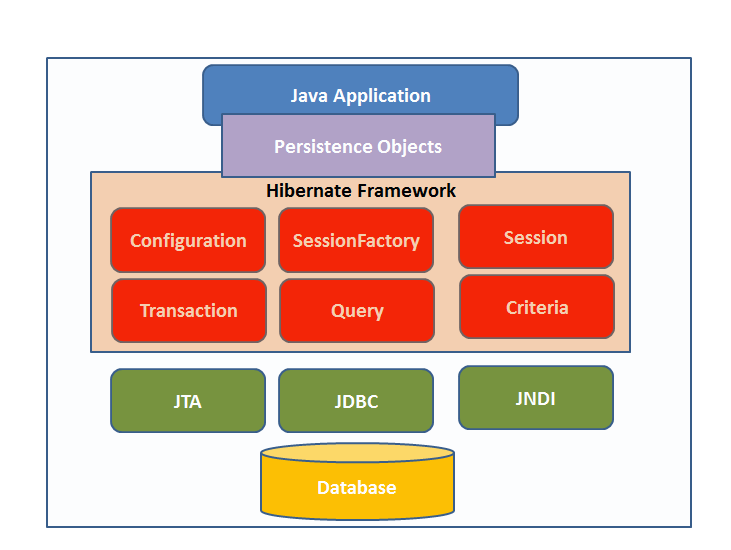
\includegraphics[scale=0.5]{hib-arch.png}%
\caption{Struttura di Hibernate}\label{fig:hibernate}%
\end{figure}

L'oggetto Configuration \`e di fondamentale importanza per il funzionamento del framework, in quanto contiene informazioni che riguardano:
\begin{itemize}
\item la connessione al database
\item il class mapping
\end{itemize}
la prima viene gestita mediante il file di configurazione hibernate.cfg.xml, mentre il mapping tra le classi java e le tabelle del database, pu\`o avvenire mediante file di configurazione xml, oppure con il meccanismo delle annotation. 

\FloatBarrier
\begin{figure}[!htb]
\centering%
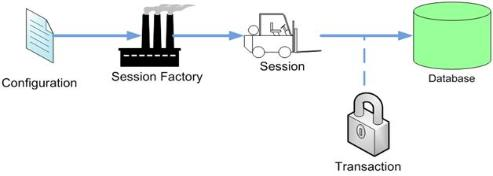
\includegraphics[scale=0.7]{hiber-arch2.jpg}%
\caption{Workflow Hibernate}\label{fig:hibernate2}%
\end{figure}

Questo oggetto viene creato una sola volta all'atto della inizializzazione della applicazione,

\begin{lstlisting}
Configuration config = new Configuration().configure("/it/resources/hibernate.cfg.xml");
\end{lstlisting}

e dopo che \`e stato utilizzato per la creazione di un altro oggetto, il SessionFactory, resta inutilizzato.

\begin{lstlisting}
SessionFactory sessionFactory = config.buildSessionFactory();
\end{lstlisting}

Quest'ultimo quindi, viene anch'esso creato una sola volta allo startup, ma a differenza di Configuration, viene utilizzato in tutta l'applicazione. L'oggetto SessionFactory \`e thread safe, ed \`e utilizzato da tutti i thread dell'applicazione, inoltre siccome dipende da Configuration, che a sua volta si riferisce ad uno specifico database, potr\`a puntare solo a quel database. Nel caso di connessioni a database multipli, avremmo mulipli Configuration e quindi multipli SessionFactory, uno per ogni Configuration.
Il SessionFactory, come si evince dal nome, risulta essere uno stampo da cui creare gli oggetti Session, necessari ogni qualvolta occorre effettuare una interazione con il database. Quando con un oggetto di questo tipo viene aperta una sessione di lavoro,

\begin{lstlisting}
Session session = sessionFactory.openSession();
\end{lstlisting}

viene stabilita una connessione fisica con il database, e siccome non \`e thread safe, dopo aver effettuato le operazioni necessarie, occorre poi chiuderla manualmente, in modo da non mantenere connessioni aperte inutilmente.
Se durante una sessione di lavoro, occorre fare operazioni di modifica sul database, come inserimenti, aggiornamenti o cancellazioni, occorre gestirle come transazioni: a tal proposito l'oggetto Session viene a sua volta utilizzato per la creazione di oggetti Transaction. 
In Hibernate le transazioni sono gestite dal TransactionManager che permette allo sviluppatore di astrarsi dal livello sottostante (JDBC, JTA, ecc.) evitando di scrivere codice specifico. Infine Query e Criteria sono utilizzati per recuperare oggetti persistenti. Gli oggetti Query utilizzano SQL oppure HQL (Hibernate Query Language) per il recupero di dati dal database e per la creazione di oggetti, mentre Criteria utilizza oggetti per la costruzione e la esecuzione di una richiesta di recupero dati. 

\section{Framework GWT}
La necessit\`a di creare un'applicazione Web nasce dai molteplici vantaggi che le applicazioni RIA ( Rich Internet Application ) possiedono nei confronti delle tecnologie alternative. Infatti rispetto alle applicazioni desktop, non richiedono installazione, gli aggiornamenti sono automatici, sono indipendenti dalla piattaforma utilizzata, pi\`u sicure in quanto girano nel ristretto ambiente del Web browser e maggiormente scalabili perch\`e la maggior parte del lavoro computazionale viene eseguito dal server.\\
Con l'avvento della tecnologia Ajax (Asynchronous JavaScript and XML), lo sviluppo di applicazioni Web si basa su uno scambio di dati in background fra Web browser e server, che
consente l'aggiornamento dinamico di una pagina Web senza eplicito ricaricamento da parte dell'utente. Purtroppo, scrivere applicazioni Ajax \`e molto complicato e perci\`o particolarmente esposto ad errori e bug; questo perch\`e JavaScript \`e un linguaggio piuttosto differente da Java e richiede molta pratica per lo sviluppo; il tutto \`e peggiorato dal fatto che JavaScript tende ad avere differenze in base al browser Web utilizzato, concentrando gli sforzi ed il tempo degli sviluppatori pi\`u sulla parte grafica che sulla logica applicativa. Google Web Toolkit (GWT) nasce proprio per risolvere questi problemi, fornendo un vero e proprio livello di astrazione che nasconde il codice JavaScript e provvede automaticamente ad uniformare le differenze tra i browser. \\
Rilasciato da Google nell'estate 2006 sotto licenza Apache, Google Web Toolkit \`e un set di tool open source che permette agli sviluppatori Web di creare e gestire complesse applicazioni fronted JavaScript scritte in Java. Il codice sorgente Java pu\`o essere compilato su qualsiasi piattaforma con i file Ant inclusi. I punti di forza di GWT sono la riusabilit\`a del codice, la possibilit\`a di realizzare pagine Web dinamiche mediante le chiamate asincrone di Ajax, la gestione delle modifiche, il bookmarking, l'internazionalizzazione e la portabilit\`a fra i differenti browser. 
\subsection{Architettura GWT 2.7}
GWT \`e caratterizzato da tre componenti base:
\begin{enumerate}
\item Un compilatore Java-JavaScript di alta qualit\`a.
\item La Java Runtime Enviroment (JRE) Emulation library.
\item Interfaccia utente
\end{enumerate}
\subsubsection*{Il compilatore}
Il compilatore Java-Javascript \`e il componente principale di GWT. Si occupa di prendere il codice Java 1.5 e produrre una versione equivalente in JavaScript ed incapsulare la varie differenze tra i browser.
Il compilatore esegue numerosi processi di ottimizzazione del codice, debugging, logging e generazione del codice.
La generazione del codice JavaScript pu\`o essere fatta con uno di questi tre stili:
\begin{description}
\item[-Offuscato]il codice \`e illeggibile, compatto e di piccole dimensioni, quindi \`e raccomandato solamente quando pubblichiamo in produzione la nostra applicazione.
\item[-Formattato]codice leggibile
\item[-Dettagliato]codice ricco di specificatori di package e signature complete: questo stile \`e molto comodo per ricavare informazioni del codice Java dalla console degli errori JavaScript.
\end{description}
\subsubsection*{JRE Emulation library}
Contiene le implementazioni in linguaggio JavaScript delle librerie Java standard maggiormente utilizzate(package java.lang.*,java.sql e java.util.*). Gli altri package(ad esempio java.io.*)sono molto limitati, includendo solo alcune interfaccie. Questa limitazione deriva dal fatto che il codice JavaScript generato da GWT viene eseguito su una sandbox del browser e stampanti.
\subsubsection*{libreria UI}
\`E una libreria User Interface contenente un insieme di interfacce e classi che permettono di disegnare le pagine web (ad es. bottoni, text boxes, immagini, ecc.). Questa \`e la libreria standard principale per creare applicazioni web-based basate su GWT.
\subsection{Comunicazione Client-Server in GWT}
\`E noto che quando si sviluppa una RIA, cosa fondamentale \`e la comunicazione tra il browser(client) e il server.
GWT fornisce differenti strade per comunicare con un server e il formato dei dati da utilizzare dipende dal server con cui si interagisce.
\subsubsection*{Utilizzando le Remote Procedure Calls(GWT RPC)}
GWT RPC \`e un framework che permette di facilitare il passaggio di oggetti Java tra client e server (e anche viceversa) attraverso il protocollo HTTP.
E' possibile utilizzare il framework GWT RPC per rendere trasparenti le
chiamate alle servlet Java e lasciare a GWT il compito di prendersi cura dei
dettagli di basso livello come la serializzazione degli oggeti.
Il meccanismo GWT RPC pu\`o esser diviso in tre parti:
\begin{enumerate}
\item Il servizio eseguito sul server
\item Il codice client che invoca il servizio
\item Gli oggetti Java trasmessi tra client e server
\end{enumerate}

\begin{figure}[htbp]
\centering%
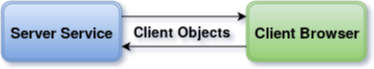
\includegraphics[scale=0.7]{RPC1.png}%
\caption{GWT RPC: interazione tra server e client mediante data object}\label{fig:rpc}}%
\end{figure}

Utilizzando GWT RPC tutte le chiamate effettuate dalla pagina HTML al server sono asincrone. Questo significa che le chiamate non bloccano il
client mentre attende una risposta dal server, ma viene eseguito il codice immediatamente successivo.
I vantaggi di effettuare chiamate asincrone rispetto alle pi\`u semplici (per gli
sviluppatori) chiamate sincrone, si riscontrano in una migliore esperienza per gli utenti finali.  innanzitutto, l'interfaccia utente \`e pi\`u reattiva; infatti,
a causa del fatto che nei browser Web il motore JavaScript \`e generalmente di
tipo single-thread, una chiamata sincrona al server genera un "blocco" fino alla conclusione della stessa, rovinando cos\`i l'esperienza dell'utente finale.
Altro vantaggio delle chiamate asincrone \`e che risulta possibile eseguire altri
lavori in attesa della risposta da parte del server; Ultimo vantaggio , ma non meno
importante, \`e che \`e possibile effettuare chiamate multiple al server nello
stesso tempo; tuttavia questo parallelismo risulta fortemente limitato dal
piccolo numero di connessioni che in genere i browser concedono alle singole
applicazioni.\\
I tipi di dato di scambio tra server e client devono essere innanzi tutto serializzabili e possono essere sostanzialmente dei seguenti tipi:
\begin{itemize}
\item Tipi primitivi Java.
\item I wrapper dei tipi primitivi
\item Un sottoinsieme degli oggetti Java Runtime Environemnt (JRE)
\item Qualsiasi tipo definito dall'utente a patto che sia serializzabile\footnote{Le chiamate alle GWT-RPC sono tra codice Javascript e Java e GWT prevede la serializzazione come parte del meccanismo RPC} 
(implementi l'interfaccia Serializable o IsSerializable di GWT)
\end{itemize}

\subsubsection*{Ricevendo dati JSON via HTTP}
Se l'applicazione comunica con un server che non pu\`o ospitare servlet Java, oppure con uno che utilizza gi\`a un'altro formato di dati come JSON o XML, si possono eseguire richieste HTTP per ottenere i dati. GWT fornisce classi HTTP generiche che possono essere utilizzate per fare le richieste, e classi XML e JSON client utilizzabili per processare le risposte.\\
Se si crea un'applicazione che richiede dati da uno o pi\`u web server remoti bisogna evitare le restrizioni SOP(Same Origin Policy)\footnote{Same Origin Policy \`e una misura di sicurezza del browser che limita il codice JavaScript client-side nell'interagire con risorse originate da nomi di dominio, porte e protocolli differenti.}.

\section{Librerie}
\subsubsection*{Apache Batik}
\subsubsection*{Vectomatic lib-gwt-svg}

\chapter{La Webapp GESTIONE AULE}
In questa sezione viene descritta l'architettura e le funzionalità del progetto, dividendo la parte server da quella client.
\begin{figure}[!htb]
\centering%
\includegraphics[scale=0.5]{MainPackDiag.png}%
\caption{Suddivisione principale del progetto}\label{fig:umlPackDiag}%
\end{figure}

Come si può notare dalla figura \ref{fig:umlPackDiag}, il progetto è stato suddiviso in due cartelle principali, una cartella contiene la parte di codice eseguita lato client dal browser web, mentre 
l’altra contiene la parte di codice eseguita lato server dall’application server Tomcat.
\section{Pattern architetturale MVP}
\FloatBarrier
\subsection{Pattern architetturale MVP}

Un' importante fase durante la progettazione di applicazioni software \`e la scelta di un'opportuna architettura, che definisce le linee guida allo sviluppo del progetto. Definire bene tale processo \`e utile sia per standardizzare il modello di sviluppo del progetto corrente, sia per le applicazioni
future.
L'impiego di un adeguato pattern porta numerosi vantaggi tra cui:
\begin{itemize}
\item Incrementa il riutilizzo del codice.
\item Facilita il lavoro in team e la pianificazione del progetto, dividendo
quest'ultimo in componenti indipendenti delegabili a gruppi di lavoro
differenti.
\item Aiuta la manutenzione del codice.
\item Aumenta la flessibilit\`a delle applicazioni e incrementa della scalabilit\`a.
\end{itemize}
Il Model-View-Presenter (MVP) \`e un pattern architetturale usato principalmente quando si vogliono creare User Interfaces. 
Il pattern MVP Separa la parte di gestione dei dati di un'applicazione dalla loro visualizzazione e manipolazione attraverso l'interfaccia utente. 
\begin{figure}[htbp]
\centering%
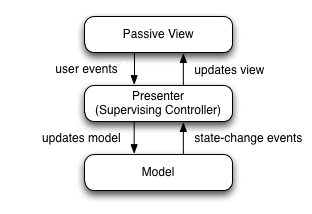
\includegraphics[scale=0.7]{MVP.png}%
\caption{Diagramma del Model-View-Presenter MVP}\label{fig:mvp}%
\end{figure}\\
Questo pattern \`e composto da tre elementi:
\begin{description}
\item[Model] \`e un'interfaccia che definisce i dati da visualizzare ed incapsula lo stato dell'applicazione.
\item[View] \`e un'interfaccia responsabile della visualizzazione dei
dati e delle informazioni, raccoglie gli input dell'utente e mai la manipolazione dei dati avviene in maniera diretta ma sempre attraverso un'interfaccia. Questo tipo di approccio consente di gestire facilmente eventuali modifiche alla GUI (Graphical User Interface) che non richiederanno mai l'aggiornamento del presenter.
\item[Presenter]  \`e colui che, oltre ad aggiornare la vista, interagisce con il model,che pu\`o essere identificato sia come lo stato di un oggetto che come dati persistenti in un'applicazione, in base alle richieste ricevute dalla view.
\end{description}
Nelle viste vi \`e una relazione uno a uno con i presenters e ci\`o permette a questi di osservare le loro viste e reagire agli eventi. Siccome le viste non possono interagire direttamente con altre viste, i presenters devono scambiare i dati con gli altri presenters. Per ottenere tale comunicazione  fra presenters, si fa uso dell' Event Bus, un oggetto in grado di trasmettere e filtrare le notifiche(figura \ref{fig:mvpEB}).

\FloatBarrier
\begin{figure}[!htb]
\centering%
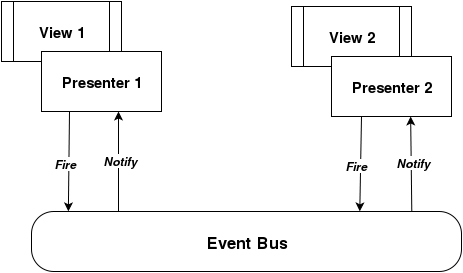
\includegraphics[scale=0.5]{EBdiagram.png}%
\caption{Comunicazione tra unit\`a del software che non sono direttamente collegate tra loro. Ognuna di esse pu\`o inviare eventi all'Event Bus ed essere in "ascolto" di  particolari eventi.}\label{fig:mvpEB}%
\end{figure}

\FloatBarrier
\begin{figure}[!htb]
\centering
\includegraphics[scale=0.45,angle=270]{GWTappMVP.png}
\caption{Implementazione client seguendo pattern MVP}
\label{fig:mvpApp}
\end{figure}



\chapter{L'applicazione MONITORAGGIO AULE}
\section{Stile architetturale REST}
Il Web è popolato da articoli e trattazioni relative alle architetture REST che tristemente ripetono le medesime battute. Pertanto, al fine di minimizzare la monotonia, in questo paragrafo ci limiteremo a ricordare brevemente i concetti fondamentali, riducendo al minimo la ripetizione delle storielle ormai usurate. L’acronimo REST, REpresentational State Transfer (“trasferimento dello stato di rappresentazione”) deriva dalla tesi di dottorato di Roy Fielding intitolata “Architectural Styles and the Design of Network-based Software Architectures” (“stili architetturali e progettazione di architetture software basate sul networking”) [2]; concediamoci una battuta ricorrente: per essere una tesi di dottorato, non è poi così difficile da leggere. Fielding è uno dei principali autori di del protocollo HTTP, HypertText Transfer Protocol, (“protocollo di trasferimento degli ipertesti”) versione 1.0 e 1.1.

REST non è un’architettura bensì uno “stile architetturale” formato da vincoli, linee guida e best practice. La formulazione dello stile REST è stata ottenuto dopo un’attenta analisi effettua da Fielding sulle risorse e le tecnologie disponibili per la creazione di applicazioni distribuite. L’assioma di base è che, senza imporre alcun vincolo, i sistemi tendono “naturalmente” a evolvere in maniera entropica, generando le conseguente negative che tutti noi ben conosciamo (sistemi costosi da creare, difficili da mantenere e da far evolvere, etc.).

Con questo assunto in mente, Fielding ha iniziato la sua esplorazione nel dominio degli stili delle architetture distribuite partendo dal limite inferiore da lui definito “spazio nullo” (null space), ossia il “Far West”, rappresentato da organizzazioni dotate di sistemi a basso grado di maturità in cui tutte le risorse tecnologiche sono disponibili, tutti gli stili sono ammessi, senza regole ne’ limiti. Continuando lungo la direttrice evolutiva, Fielding ha poi definito lo stato di totale maturità caratterizzato da sistemi che rispettano le regole da lui definite e che quindi possono essere definiti compatibili con le guideline REST (RESTful). Queste regole sono condensate nei seguenti sei vincoli, di cui i primi cinque sono obbligatori, mentre l’ultimo è facoltativo. Vediamo quindi i 5+1 vincoli cui un sistema deve sottostare per essere definito RESTful.


\chapter{Conclusioni}
Mi ritengo soddisfatto del progetto di tesi svolto.
Innanzitutto, sono stati affrontati
problemi pratici che riguardano la produzione di software, sia dal lato progettuale sia da quello implementativo.
L'adozione di frameworks è risultata molto efficacie, rendendo lo sviluppo del software più semplice permettendo la creazione di una struttura  adattabile e flessibile risolvendo in tal modo numerose problematiche.\\
GWT ha permesso di trasformare trasparentemente e automaticamente il codice prodotto in una RIA Ajax con tanto di client che lavora in modalità asincrona direttamente dentro il browser senza preoccuparsi del codice JavaScript.
Inoltre, grazie al pattern design adottato, abbiamo potuto lavorare efficacemente in team. \\
Hibernate ha permesso di ridurre significativamente i tempi  di sviluppo altrimenti impiegati in attività manuali di gestione dei dati in SQL e JDBC risolvendo problemi legati all'impedence mismatch e riducendo significativamente la quantità di codice per la persistenza rendolo altamente manutenibile.
La scelta di utilizzare immagini vettoriali SVG ha permesso un ampia manipolazione di esse grazie all'ausilio di librerie open source e rendendo l'interfaccia con l'utente intuitiva ed esteticamente gradevole.

\begin{thebibliography}{99}
\bibitem{hibernate} 
Christian Bauer, Gavin King;
\textit Java Persistence with Hibernate
\bibitem{gwt} 
Adam Tacy, Robert Hanson, Jason Essington, Anna Tokke;
\textit GWT in Action
\end{thebibliography}

\end{document}